\clearpage
\chapter{Lexical analyzer for C language using C language}

\section{Aim}
To design and implement a lexical analyzer for given language using C. The lexical analyzer should ignore redundant spaces, tabs and new lines.

\section{Algorithm}

\begin{figure}[H]
	\centering
	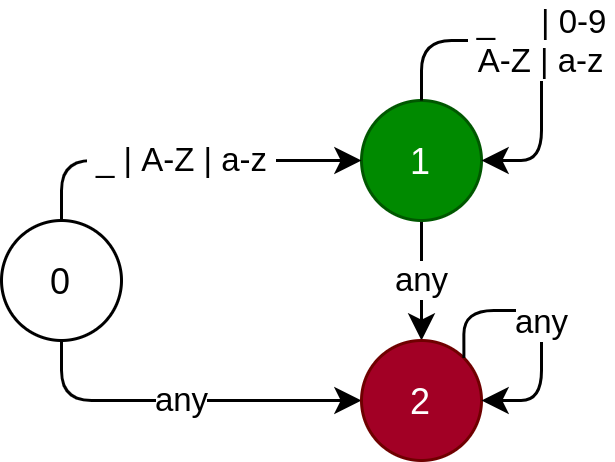
\includegraphics[height=2.5in]{../EXP1/identifier.png}
	\caption{Finite Automaton to detect an identifier.}
\end{figure}

\begin{figure}[H]
	\centering
	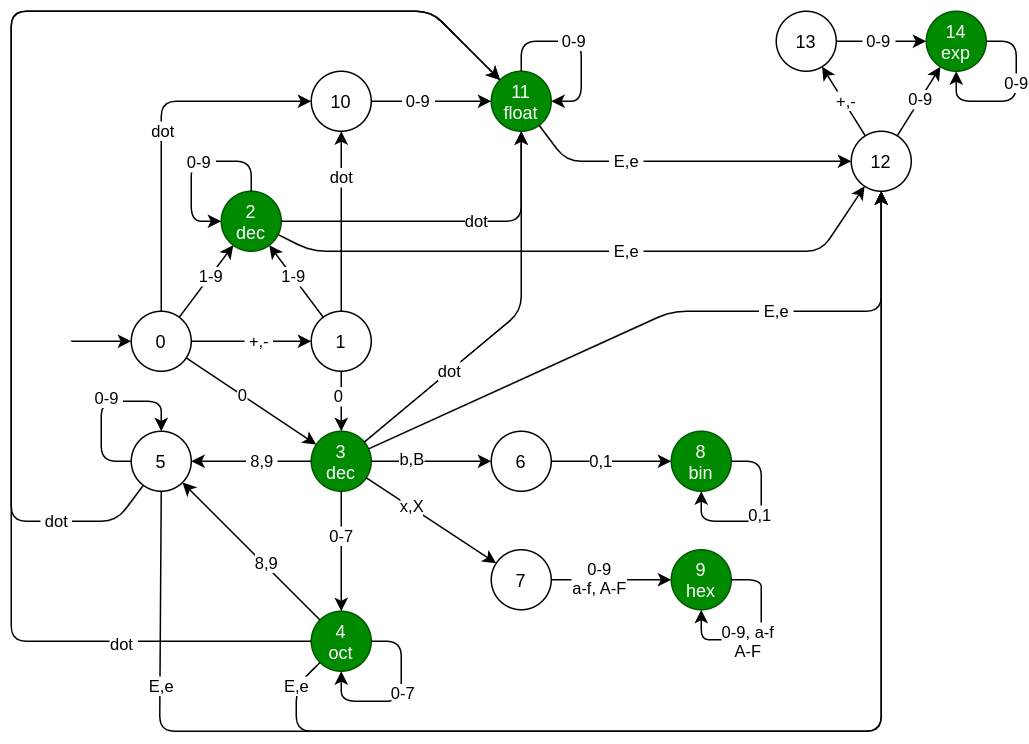
\includegraphics[width=\textwidth]{../EXP1/numerals.png}
	\caption{Finite Automaton to detect an numeral type.}
\end{figure}


\begin{figure}[H]
	\centering
	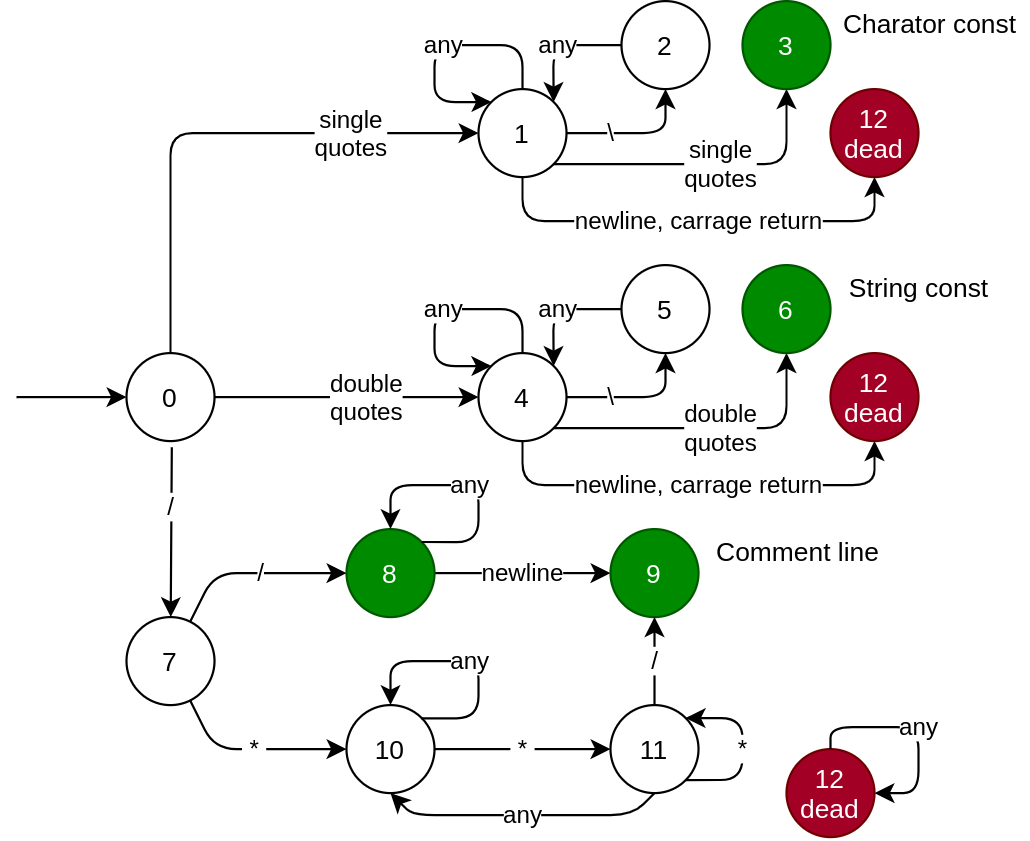
\includegraphics[width=\textwidth]{../EXP1/char-stream.png}
	\caption{Finite Automaton to detect comments, string/char literal and escape sequence}
\end{figure}


\section{C-Program}
Header file \textbf{stack.h} to stimulate stack.
\lstinputlisting[style=CStyle]{../EXP1/stack.h}

\vspace{0.5cm}
Header file \textbf{definition.h} holds various subroutines and constants that aid to analyze lexemes of C language.
\lstinputlisting[style=Cstyle]{../EXP1/definition.h}

\vspace{0.5cm}
C program file \textbf{CLexical.c} initiates and scans lexemes.
\lstinputlisting[style=Cstyle]{../EXP1/CLexical.c}


\section{Output}
C program used for testing \textbf{sample.c}.
\lstinputlisting[style=CStyle]{../EXP1/sample.c}

\vspace{0.5cm}
Lexical analyzer output
\lstinputlisting[style=plain]{../EXP1/sample_out.txt}

\section{Result}
The program compiled successfully and identified various C tokens from the sample C program file.